\documentclass[8pt]{beamer}
\usetheme{default} % Very simple theme
\usecolortheme{dove} % Minimalist grayscale colors
\setbeamertemplate{navigation symbols}{} % Remove navigation bar

% Define brand-like colors
\definecolor{myblue}{RGB}{0, 102, 204}    % Blue for standard blocks
\definecolor{mygreen}{RGB}{0, 153, 0}     % Green for example blocks
\definecolor{myred}{RGB}{204, 0, 0}       % Red for alert blocks
\definecolor{myorange}{RGB}{255, 128, 0} % For \emph

% Accent color for titles, bullets, etc.
\setbeamercolor{structure}{fg=myblue}

% Block colors
\setbeamercolor{block title}{bg=myblue, fg=white}
\setbeamercolor{block body}{bg=blue!5, fg=black}

\setbeamercolor{exampleblock title}{bg=mygreen, fg=white}
\setbeamercolor{exampleblock body}{bg=green!5, fg=black}

\setbeamercolor{alertblock title}{bg=myred, fg=white}
\setbeamercolor{alertblock body}{bg=red!5, fg=black}
\setbeamercolor{alerted text}{fg=myred}

% Optional: color for \example text
\setbeamercolor{example text}{fg=mygreen}

% Custom emph (orange text instead of italic)
\let\oldemph\emph
\renewcommand{\emph}[1]{\textcolor{myorange}{#1}}
\newcommand{\ve}[1]{\boldsymbol{#1}}

\usepackage{graphicx} % Package for images
\usepackage{amsmath} % Package for images
\graphicspath{{figs/}} % Path to your figures directory
\usepackage{array}  % For better column spacing
\usepackage{caption} % Required for \captionof
\usepackage{tikz}
\usetikzlibrary{arrows.meta,positioning,shapes.geometric}
%\usepackage{enumitem}

% Title Information
\title{STOCHASTIC METHODS IN WATER RESOURCES}
\vspace{25pt}
\subtitle{Unit 6: Stochastic modelling and prediction \\ Lecture 20: Introduction to Kalman filter}
\author{Luis Alejandro Morales, Ph.D.}
\institute{Universidad Nacional de Colombia \\ Department of Civil and Agriculture Engineering} %// }
%\date{\today}

\begin{document}

% Title Slide
\begin{frame}
    \titlepage
\end{frame}

% Slide 2
% \begin{frame}{Outline}
% \tableofcontents
% \end{frame}

\section{Introduction and Applications}

% Slide 3
\begin{frame}{Kalman Filter in Hydrology: Overview}
\begin{itemize}
\item Recursive algorithm for optimal state estimation in linear dynamic systems
\item Minimizes posterior estimation error variance (Minimum Mean Square Error (MMSE) estimator)
\item Combines:
  \begin{itemize}
  \item Model prediction (hydrological process model)
  \item Noisy observations (gauges, satellites)
  \end{itemize}
\item Typical hydrological applications:
  \begin{itemize}
  \item Streamflow forecasting
  \item Flood warning systems
  \item Groundwater level estimation
  \item Soil moisture assimilation
  \end{itemize}
\item Particularly useful when observations are sparse and uncertain
\end{itemize}

\vspace{0.3cm}
\textbf{Conceptual flow:}
\begin{center}
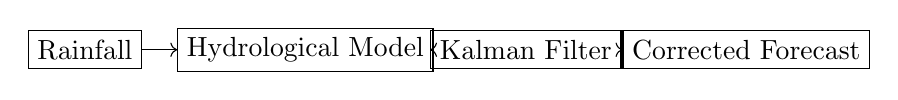
\begin{tikzpicture}[node distance=2.8cm]
\node (rain) [draw, rectangle] {Rainfall};
\node (model) [draw, rectangle, right of=rain] {Hydrological Model};
\node (kf) [draw, rectangle, right of=model] {Kalman Filter};
\node (out) [draw, rectangle, right of=kf] {Corrected Forecast};
\draw[->] (rain) -- (model);
\draw[->] (model) -- (kf);
\draw[->] (kf) -- (out);
\end{tikzpicture}
\end{center}
\end{frame}

\section{Mathematical Framework}

% Slide 4
\begin{frame}{State-Space Representation and Assumptions}
\textbf{System (Process) Model}
\begin{equation}
\mathbf{x}_k = A\mathbf{x}_{k-1} + B\mathbf{u}_k + \mathbf{w}_k
\end{equation}

\textbf{Measurement Model}
\begin{equation}
\mathbf{z}_k = H\mathbf{x}_k + \mathbf{v}_k
\end{equation}

\textbf{Definitions:}
\begin{itemize}
\item $\mathbf{x}_k$ : State vector (e.g. discharge, water table, soil moisture)
\item $A$ : State transition matrix
\item $H$ : Observation operator
\item $\mathbf{w}_k \sim N(0,Q)$ : Process noise
\item $\mathbf{v}_k \sim N(0,R)$ : Observation noise
\end{itemize}

\textbf{Assumptions:}
\begin{itemize}
\item Linearity
\item Gaussian, white, zero-mean noise
\item Known covariance matrices $Q$, $R$
\end{itemize}
\end{frame}

\section{Kalman Filter Algorithm}

% Slide 5
\begin{frame}{Kalman Filter Equations (Prediction + Update)}
\textbf{Prediction Step}
\begin{align}
\hat{x}_{k|k-1} &= A\hat{x}_{k-1|k-1} \\
P_{k|k-1} &= A P_{k-1|k-1} A^T + Q
\end{align}

\textbf{Update Step}
\begin{align}
K_k &= P_{k|k-1} H^T (H P_{k|k-1} H^T + R)^{-1} \\
\hat{x}_{k|k} &= \hat{x}_{k|k-1} + K_k(z_k - H\hat{x}_{k|k-1}) \\
P_{k|k} &= (I - K_k H) P_{k|k-1}
\end{align}

\textbf{Interpretation:}
\begin{itemize}
\item $K_k$ balances model confidence vs observation reliability
\item Innovation: $z_k - H\hat{x}_{k|k-1}$ = new information
\end{itemize}
\end{frame}

\section{Hydrological Case Studies}

% Slide 6
\begin{frame}{Case Study 1: Flood Routing (Muskingum Model)}
\textbf{State:} Channel storage and discharge

Muskingum routing in state-space form:
\begin{equation}
Q_{k+1} = a Q_k + b I_k + w_k
\end{equation}

Measurement:
\begin{equation}
z_k = Q_k + v_k
\end{equation}

\begin{itemize}
\item $Q_k$ : Channel discharge
\item $I_k$ : Inflow
\item Kalman Filter corrects predicted hydrograph in real-time
\item Used in flood early-warning systems
\end{itemize}

\textbf{Outcome:}
\begin{itemize}
\item Reduced peak error
\item Improved lead time estimation
\end{itemize}
\end{frame}

% --- Simple Example: Kalman Filter + Muskingum Flood Routing ---
\begin{frame}{Simple Example: Kalman Filter for Flood Routing (Muskingum Model)}
\textbf{Objective:} Improve flood routing discharge prediction using real-time observations.

\medskip
\textbf{Muskingum routing equation (discrete):}
\[
Q_{out}(k+1) = C_1 Q_{in}(k+1) + C_2 Q_{in}(k) + C_3 Q_{out}(k)
\]

Coefficients:
\[
C_1 = \frac{\Delta t - 2KX}{2K(1-X)+\Delta t}, \quad
C_2 = \frac{\Delta t + 2KX}{2K(1-X)+\Delta t}, \quad
C_3 = \frac{2K(1-X)-\Delta t}{2K(1-X)+\Delta t}
\]

where $K$ is the travel time of the flood wave through the reach and $X$ is a weighting factor ($0 \leq X \leq 0.5$)

\textbf{State variable:}
\[
x_k = Q_{out}(k)
\]

State-space form:
\[
x_{k+1} = C_3 x_k + C_1 u_{k+1} + C_2 u_k + w_k
\]
\[
z_k = x_k + v_k
\]

\textbf{Kalman Filter Steps:}

\textbf{Prediction:}
\[
\hat{x}_{k+1|k} = C_3 \hat{x}_{k|k} + C_1 u_{k+1} + C_2 u_k
\]
\[
P_{k+1|k} = C_3^2 P_{k|k} + Q
\]

\textbf{Update:}
\[
K_{k+1} = \frac{P_{k+1|k}}{P_{k+1|k}+R}
\]
\[
\hat{x}_{k+1|k+1} = \hat{x}_{k+1|k} + K_{k+1}(z_{k+1}-\hat{x}_{k+1|k})
\]
\[
P_{k+1|k+1} = (1-K_{k+1})P_{k+1|k}
\]
\end{frame}

\begin{frame}{Simple Example: Kalman Filter for Flood Routing (Muskingum Model)}
\textbf{Hydrological Interpretation:}
\begin{itemize}
\item Model propagates flood wave downstream.
\item Kalman Filter corrects routing using observed hydrograph.
\item Improves peak timing and magnitude prediction.
\item Essential for operational flood forecasting.
\end{itemize}
\end{frame}

% Slide 7
\begin{frame}{Case Study 2: Groundwater Level Estimation}
\textbf{State Vector}
\begin{equation}
\mathbf{x}_k = [h_k]
\end{equation}

Groundwater dynamics (linearized form):
\begin{equation}
h_{k+1} = h_k + \Delta t(\alpha R_k - \beta Q_{out}) + w_k
\end{equation}

Observation model:
\begin{equation}
z_k = h_k + v_k
\end{equation}

\begin{itemize}
\item Assimilates piezometer readings
\item Filters pumping-induced noise
\item Useful in aquifer management
\end{itemize}

\textbf{Benefit:} Stable groundwater trend estimation under uncertainty
\end{frame}

% Slide 8
\begin{frame}{Case Study 3: Soil Moisture Assimilation}
\textbf{State:} Root-zone soil moisture content

Bucket model:
\begin{equation}
S_{k+1} = S_k + P_k - ET_k - D_k + w_k
\end{equation}

Observation from satellite:
\begin{equation}
z_k = c S_k + v_k
\end{equation}

\begin{itemize}
\item Integrates remote sensing + model simulation
\item Improves drought monitoring
\item Basis for irrigation scheduling
\end{itemize}

\textbf{Extension:} EnKF preferred for distributed soil models
\end{frame}

\section{Advanced Extensions}

% Slide 9
\begin{frame}{EKF and EnKF in Hydrology}
\textbf{Extended Kalman Filter (EKF)}
\begin{itemize}
\item Nonlinear model: $x_k = f(x_{k-1}) + w_k$
\item Linearization using Jacobians
\item Suitable for rainfall-runoff models
\end{itemize}

\textbf{Ensemble Kalman Filter (EnKF)}
\begin{itemize}
\item Represents uncertainty using ensemble of states
\item Updates each ensemble member statistically
\item Widely used in distributed hydrological models
\end{itemize}

\textbf{Comparison:}
\begin{itemize}
\item EKF: Faster but local linearization errors
\item EnKF: Computational but more robust
\end{itemize}
\end{frame}

\section{Synthesis}

% Slide 10
\begin{frame}{Benefits, Limitations and Conclusions}
\textbf{Key Benefits}
\begin{itemize}
\item Real-time data assimilation
\item Error reduction in hydrological forecasts
\item Dynamic uncertainty quantification
\end{itemize}

\textbf{Limitations}
\begin{itemize}
\item Linearity assumptions
\item Sensitivity to noise covariance selection
\item Requires continuous observations
\end{itemize}

\textbf{Conclusion}
\begin{itemize}
\item Kalman Filter is a fundamental tool in modern hydrology
\item Enables integration of physics-based models with observations
\item Essential for flood, drought and groundwater management
\end{itemize}
\end{frame}

\end{document}
